\section{Numerical Experiments}\label{section3}
Having in mind expressions (\ref{Bernoulli9buena}) and (\ref{Bernoulli10buena1}), two different approximations are given to compute cosine matrix function.\\
To test the proposed method and the two distinct approximations, and to compare them with other approaches, the following algorithms have been implemented on MATLAB R2018b:

\begin{description}
\item $\bullet$  \emph{cosmber}. New code based on the new developments of Bernoulli matrix polynomials (formulae (\ref{Bernoulli9buena}) and (\ref{Bernoulli10buena1})). The maximum value of $m$ to be used is $m=36$, with even and odd terms.
\item $\bullet$  \emph{cosmtay}. Code based on the Taylor series for the cosine \cite{sastre2017two}. It will provide a maximum value of $m=16$, considering only the even terms, which would be equivalent to $m=32$ using the even and odd terms.
\item $\bullet$   \emph{cosmtayher}. Code based on the Hermite series for the cosine \cite{defez2019efficient}. As mentioned before, it will provide a maximum value of $m=16$.
\item $\bullet$   \emph{cosm}. Code based on the Pad\'e rational approximation for the cosine \cite{AlHR15}.
\end{description}

The following sets of matrices have been used:

\begin{description}
\item[a)] \textbf{Diagonalizable matrices}. The matrices have been obtained as $A=V \cdot D \cdot V^{T}$,
where $D$ is a diagonal matrix (with complex or real values) and matrix $V$ is an orthogonal matrix, $V=H/16$, where $H$ is a Hadamard matrix.
We have $2.18 \leq \left\|A \right\|_1 \leq 207.52$. The matrix cosine is exactly calculated as $\cos{(A)}=V \cdot \cos{(D)} \cdot V^{T}$.

\item[b)] \textbf{Non-diagonalizables matrices}. The matrices have been computed as $A=V \cdot J \cdot V^{-1}$, where
$J$ is a Jordan matrix with complex eigenvalues with module less than $10$ and random algebraic multiplicity between $1$ and $5$. Matrix $V$ is a random
matrix with elements in the interval $[-0.5,0.5]$. We have $1279.16 \leq \left\|A \right\|_1 \leq 87886.4$. The matrix cosine
is exactly calculated as $\cos{(A)}=V \cdot \cos{(J)} \cdot V^{-1}$.

\item[c)] \textbf{Matrices from the Matrix Computation Toolbox} \cite{higham1995test} and from the  \textbf{Eigtool Matlab package}~\cite{wright2009eigtool}. These matrices have been chosen because they have more varied and significant characteristics.
\end{description}

In the numerical test, we used $259$ matrices of size $128\times 128$: $100$ from the diagonalizable set, $100$ from the non-diagonalizable set, $42$ from Matrix Computation Toolbox and $17$ from Eigtool Matlab package. Results are given in Tables \ref{tabla_er_comparative_test_todo} and \ref{tabla_er_comparative_test_todoa}. The rows of each table show the percentage of cases in which the relative errors of \texttt{cosmber} (Bernoulli) is lower, greater or equal than the relative errors of \texttt{cosmtay} (Taylor), \texttt{cosmtayher} (Hermite)  and  \texttt{cosm} (Pad\'e). Graphics of the Normwise relative errors and the Performance Profile are given in Figures \ref{fig:todo} and \ref{fig:todoa}. The total number of matrix products was: $3202$ (\emph{cosmber}), $2391$ (\emph{cosmtay}), $1782$ (\emph{cosmtayher}) and  $3016$ (\emph{cosm}). Recall that in the Bernoulli implementation, the maximum value of $m$ to be used was $m=36$ considering all the terms and, in the rest of algorithms, was $m=32$ but just having into account the even terms.


\begin{table}[H]
\hspace{-1cm}
\begin{minipage}[b]{0.55\linewidth} %Una minipágina que cubre la mitad de la página
\centering
\begin{table}[H]\begin{center}
\caption{Using approximation (\ref{Bernoulli9buena})}
\resizebox{\textwidth}{!}{
\begin{tabular}{cc}\hline
$E(cosmber)<E(cosmtay)$ & $55.60\%$  \\\hline
$E(cosmber)>E(cosmtay)$ & $44.40\%$ \\\hline
$E(cosmber)=E(cosmtay)$  & $0\%$ \\\hline
$E(cosmber)<E(cosmtayher)$ & $50.97\%$ \\\hline
$E(cosmber)>E(cosmtayher)$ & $49.03\%$ \\\hline
$E(cosmber)=E(cosmtayher)$  & $0\%$ \\\hline
$E(cosmber)<E(cosm)$ & $76.83\%$ \\\hline
$E(cosmber)>E(cosm)$ & $23.17\%$ \\\hline
$E(cosmber)=E(cosm)$  & $0\%$ \\\hline
\end{tabular}
}
\label{tabla_er_comparative_test_todo}
\end{center}
\end{table}
\end{minipage}
\hspace{0.35cm} % Si queremos tener un poco de espacio entre las dos figuras
\begin{minipage}[b]{0.55\linewidth}
\centering
\begin{table}[H]\begin{center}
\caption{Using approximation (\ref{Bernoulli10buena1})}
\resizebox{\textwidth}{!}{
\begin{tabular}{cc}\hline
$E(cosmber)<E(cosmtay)$ & $65.64\%$ \\\hline
$E(cosmber)>E(cosmtay)$ & $34.36\%$ \\\hline
$E(cosmber)=E(cosmtay)$  & $0\%$ \\\hline
$E(cosmber)<E(cosmtayher)$ & $60.62\%$ \\\hline
$E(cosmber)>E(cosmtayher)$ & $39.38\%$ \\\hline
$E(cosmber)=E(cosmtayher)$  & $0\%$ \\\hline
$E(cosmber)<E(cosm)$ & $73.75\%$ \\\hline
$E(cosmber)>E(cosm)$ & $26.25\%$ \\\hline
$E(cosmber)=E(cosm)$  & $0\%$ \\\hline
\end{tabular}
}
\label{tabla_er_comparative_test_todoa}
\end{center}
\end{table}
\end{minipage}
\end{table}

\begin{figure}[htbp]
\centering
\subfigure[Using formula (\ref{Bernoulli9buena})]{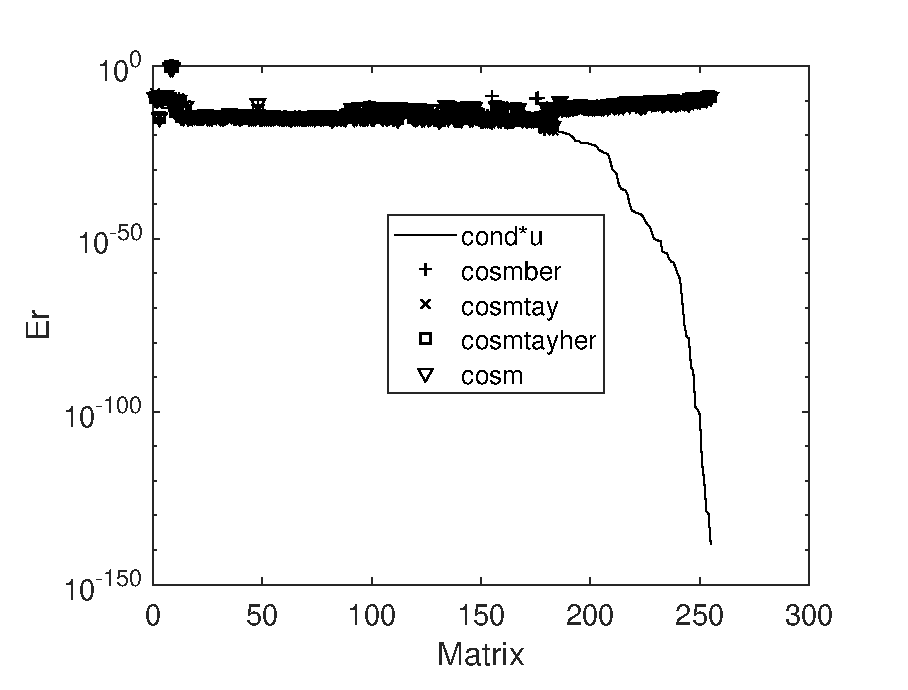
\includegraphics[scale=0.42]{Fig_normwise_9.eps}} %width=40mm
\subfigure[Using formula (\ref{Bernoulli10buena1})]{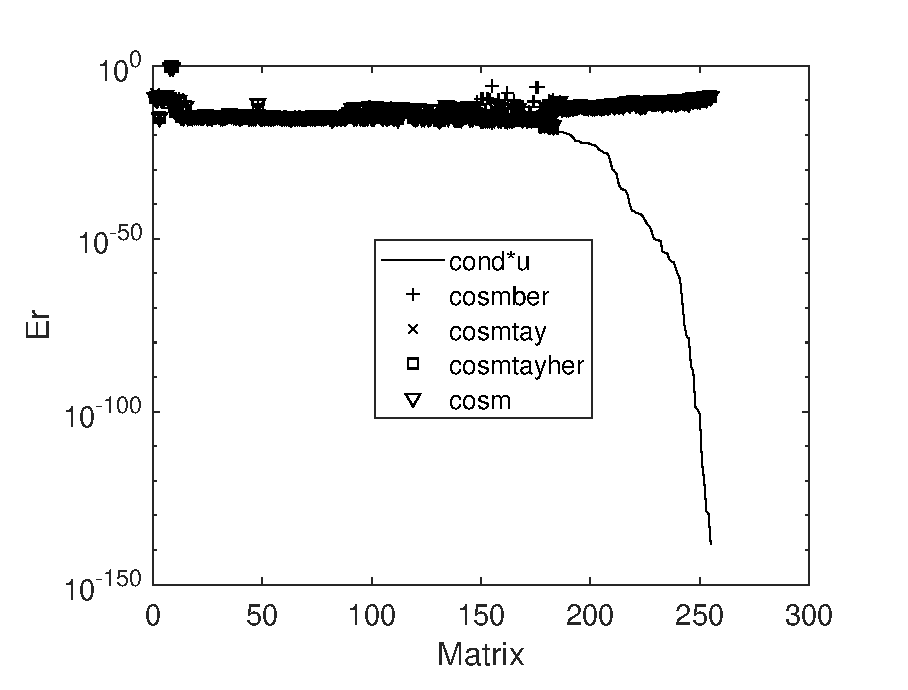
\includegraphics[scale=0.42]{Fig_todas_normwise.eps}}
\caption{Normwise relative errors.} \label{fig:todo}
\end{figure}


\begin{figure}[htbp]
\centering
\subfigure[Using formula (\ref{Bernoulli9buena})]{\includegraphics[scale=0.42]{Fig_todas_nprofile_9.eps}} %width=40mm
\subfigure[Using formula (\ref{Bernoulli10buena1})]{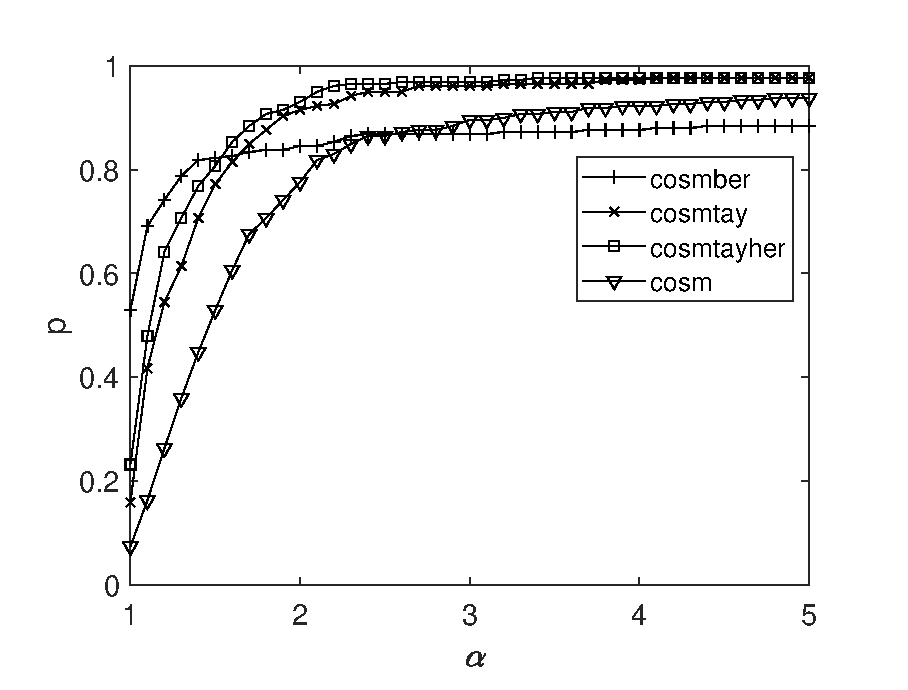
\includegraphics[scale=0.42]{Fig_todas_nprofile.eps}}
\caption{Performance Profile.} \label{fig:todoa}
\end{figure}

